\begin{minipage}[b]{0.45\linewidth}
  \centering
  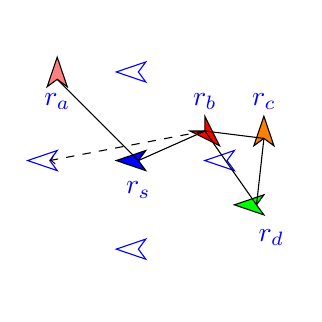
\begin{tikzpicture}[scale=0.75]
    \useasboundingbox (1,0.5) rectangle (5.5,5);
    % center 2.875 2.75
    \coordinate (S) at (2.875, 2.75);
    \def\shifty{1}
    \def\ddy{2.5}
    \coordinate (A) at (1.5, 4.125);
    \coordinate (B) at (4,4.25-\shifty);
    \draw[fill=blue] (3,2.92) -- (2.5,2.75) -- (3,2.58) -- (2.875,2.75) -- cycle;
    \def\offset{0.5}
    \node[color=blue] at (2.875, 2.75-\offset) {$r_s$};
    % vacancies
    \def\dx{1.5}
    \def\dy{1.5}
    \draw[color=blue] (3+\dx,2.92) -- (2.5+\dx,2.75) -- (3+\dx,2.58) -- (2.875+\dx,2.75) -- cycle;
    \draw[color=blue] (3-\dx,2.92) -- (2.5-\dx,2.75) -- (3-\dx,2.58) -- (2.875-\dx,2.75) -- cycle;
    \draw[color=blue] (3,2.92+\dy) -- (2.5,2.75+\dy) -- (3,2.58+\dy) -- (2.875,2.75+\dy) -- cycle;
    \draw[color=blue] (3,2.92-\dy) -- (2.5,2.75-\dy) -- (3,2.58-\dy) -- (2.875,2.75-\dy) -- cycle;
    % another two robots
    \draw[fill=red!50] (1.5,4.5) -- (1.33,4) -- (1.5,4.125) -- (1.67,4) -- cycle; % center .5 4.125
    \node[color=blue] at (1.5, 3.25+\offset) {$r_a$};
    \draw[fill=red] (4.25,4-\shifty) -- (4,4.5-\shifty) -- (4,4.25-\shifty) -- (3.75,4.25-\shifty) -- cycle; % center 3.75 4.25
    \node[color=blue] at (4, 4.75-\shifty) {$r_b$};
    \draw[] (S) -- (A);
    \draw[] (S) -- (B);
    \coordinate (V) at (2.875-\dx,2.75);
    \draw[dashed, ->] (B) -- (V);
    % two children of r_b
    \coordinate (C) at  (5, 3.125);
    \draw[fill=orange] (5,3.5) -- (4.83,3) -- (5, 3.125) -- (5.17,3) -- cycle; % center .\5 3.625
    \node[color=blue] at (5, 3.75) {$r_c$};
    \draw[] (B) -- (C);
    \coordinate (D) at (5.375-\offset, 4.5-\ddy);
    \draw[fill=green] (5.5-\offset,4.67-\ddy) -- (5-\offset,4.5-\ddy) -- (5.5-\offset,4.33-\ddy) -- (5.375-\offset,4.5-\ddy) -- cycle;
    \node[color=blue] at (5.125, 3.95-\ddy) {$r_d$};
    \draw[] (B) -- (D);
    \draw[] (C) -- (D);
  \end{tikzpicture}
\end{minipage}
\begin{minipage}[b]{0.45\linewidth}
  \centering
  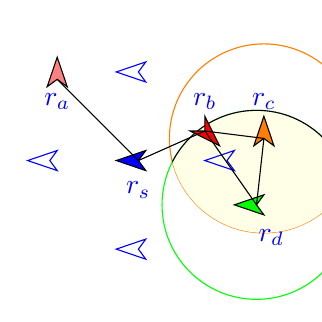
\begin{tikzpicture}[scale=0.75]
    \useasboundingbox (1,0.5) rectangle (5.5,5);
    % center 2.875 2.75
    \coordinate (S) at (2.875, 2.75);
    \def\shifty{1}
    \def\ddy{2.5}
    \def\offset{0.5}
    \coordinate (A) at (1.5, 4.125);
    \coordinate (B) at (4,4.25-\shifty);
    \coordinate (C) at  (5, 3.125);
    \coordinate (D) at (5.375-\offset, 4.5-\ddy);
     % ranges of r_c and r_d
    \def\childcircleD{(D) circle (1.6)}
    \def\childcircleC{(C) circle (1.6)}
    \draw[orange] \childcircleC;
    \draw[green] \childcircleD;
    % intersection region of children's ranges
    \begin{scope}
      \clip \childcircleC;
      \filldraw[fill=yellow!10] \childcircleD;
    \end{scope}
    
    \draw[fill=blue] (3,2.92) -- (2.5,2.75) -- (3,2.58) -- (2.875,2.75) -- cycle;
    \node[color=blue] at (2.875, 2.75-\offset) {$r_s$};
    % vacancies
    \def\dx{1.5}
    \def\dy{1.5}
    \draw[color=blue] (3+\dx,2.92) -- (2.5+\dx,2.75) -- (3+\dx,2.58) -- (2.875+\dx,2.75) -- cycle;
    \draw[color=blue] (3-\dx,2.92) -- (2.5-\dx,2.75) -- (3-\dx,2.58) -- (2.875-\dx,2.75) -- cycle;
    \draw[color=blue] (3,2.92+\dy) -- (2.5,2.75+\dy) -- (3,2.58+\dy) -- (2.875,2.75+\dy) -- cycle;
    \draw[color=blue] (3,2.92-\dy) -- (2.5,2.75-\dy) -- (3,2.58-\dy) -- (2.875,2.75-\dy) -- cycle;
    % another two robots
    \draw[fill=red!50] (1.5,4.5) -- (1.33,4) -- (1.5,4.125) -- (1.67,4) -- cycle; % center .5 4.125
    \node[color=blue] at (1.5, 3.25+\offset) {$r_a$};
    \draw[fill=red] (4.25,4-\shifty) -- (4,4.5-\shifty) -- (4,4.25-\shifty) -- (3.75,4.25-\shifty) -- cycle; % center 3.75 4.25
    \node[color=blue] at (4, 4.75-\shifty) {$r_b$};
    \draw[] (S) -- (A);
    \draw[] (S) -- (B);
    % two children of r_b
    \draw[fill=orange] (5,3.5) -- (4.83,3) -- (5, 3.125) -- (5.17,3) -- cycle; % center .\5 3.625
    \node[color=blue] at (5, 3.75) {$r_c$};
    \draw[] (B) -- (C);
  
    \draw[fill=green] (5.5-\offset,4.67-\ddy) -- (5-\offset,4.5-\ddy) -- (5.5-\offset,4.33-\ddy) -- (5.375-\offset,4.5-\ddy) -- cycle;
    \node[color=blue] at (5.125, 3.95-\ddy) {$r_d$};
    \draw[] (B) -- (D);
    \draw[] (C) -- (D);
   
  \end{tikzpicture}
\end{minipage}
 \caption{[left]. Let robot $r_s$ be a stable robot, it has two
   neighbors $r_a, r_b$, given the square lattice graph as input
   (Figure~\ref{fig:sq}), $r_s$ will have four vacancies. Assume $r_b$
   is the unstable robot with the highest ID, and it intends to move
   towards the vacancy ahead of $r_5$. }
